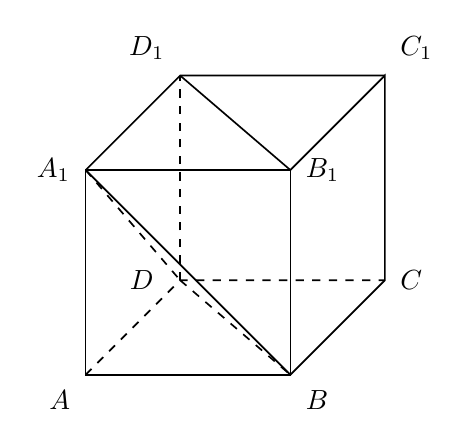
\begin{tikzpicture}[x=1cm,y=1cm,line width=.6pt]
% Cube ABCD-A1B1C1D1, front ABB1A1 square, depth (1.2,1.2)
\coordinate (A) at (0,0);
\coordinate (B) at (2.6,0);
\coordinate (B1) at (2.6,2.6);
\coordinate (A1) at (0,2.6);
\coordinate (D) at (1.2,1.2);
\coordinate (C) at (3.8,1.2);
\coordinate (D1) at (1.2,3.8);
\coordinate (C1) at (3.8,3.8);
% solid cube outline
\draw (A) -- (B) -- (B1) -- (A1) -- cycle;
\draw (B) -- (C) -- (C1) -- (B1);
\draw (A1) -- (D1) -- (C1);
\draw (A1) -- (B1);
% pyramid base BB1D1D top diagonal + apex diagonals
\draw (D1) -- (B1);
\draw (A1) -- (B);
% dashed hidden + base diagonal
\draw[dashed] (A) -- (D) -- (C);
\draw[dashed] (D) -- (D1);
\draw[dashed] (A1) -- (D);
\draw[dashed] (D) -- (B);
% labels
\node[below left=2pt] at (A) {$A$};
\node[below right=2pt] at (B) {$B$};
\node[right=2pt] at (C) {$C$};
\node[left=6pt] at (D) {$D$};
\node[left=2pt] at (A1) {$A_{1}$};
\node[right=2pt] at (B1) {$B_{1}$};
\node[above right=2pt] at (C1) {$C_{1}$};
\node[above left=2pt] at (D1) {$D_{1}$};
\end{tikzpicture}
